\documentclass{article}

\usepackage[scaled]{helvet}
\renewcommand\familydefault{\sfdefault} 
\usepackage[T1]{fontenc}
\usepackage{fancyhdr}
\usepackage{graphicx}
\usepackage{subfigure}
\usepackage{booktabs}
\usepackage[inline]{enumitem}

\usepackage{amsmath}
\usepackage{hyperref}
\hypersetup{
    colorlinks=true,
    citecolor=[RGB]{0,0.5,0.5},
    urlcolor=[RGB]{0,0.5,0.5},
    linkcolor=[RGB]{0,0.5,0.5}
}

\usepackage{geometry}
\geometry{margin={0.8in,1in}}

\usepackage[colorinlistoftodos,prependcaption,textsize=small]{todonotes}

\usepackage{minted}
\fancyfoot[L]{\href{https://www.example.com}{Click Here for Example}} 

\begin{document}

\begin{centering}
\Large\textbf{{\sc CMPT 423-820 Mini Project 2 Report}}\\[1ex]
\begin{center}
\small{Alireza Falamarzi (ylw576), Baptiste Rouquette (dly490), Princess Tayab (prt898), Talha Mansoor (kgy284)}
\end{center}
\end{centering}
\hrule


\section{The Loss Objective}
We have used the sum of cross-entropy loss as our loss objective. By minimizing this summed loss, we maximize the likelihood of the correct class. Given a dataset \( D = \{ (x_{i}, y_{i}) \}_{i=1}^{D} \), where each image \( x_i \) is labeled with a formula \( y_i \) (3 characters: digit + operator + digit), we label each image as \( y_i = (y_{i1}, y_{i2}, y_{i3}) \), with \( y_{i1} \) representing the first digit, \( y_{i2} \) the operator, and \( y_{i3} \) the second digit. The likelihood of the dataset \( D \) given the parameters \( \theta \) is then:

\begin{equation}
L(\theta) = \prod_{i=1}^{D} P(y_i \mid x_i; \theta)
\end{equation}

\noindent where \( y_i = (y_{i1}, y_{i2}, y_{i3}) \) represents the true labels for the first digit, operator, and second digit. Now we use the log trick  to turn the product into a sum:
\begin{equation}
\log L(\theta) = \sum_{i=1}^{D} \left[ \log P(y_{i1} \mid x_i; \theta) + \log P(y_i \mid x_i; \theta) + \log P(y_{i3} \mid x_i; \theta) \right]
\end{equation}
And then to convert the maximization problem into a minimization problem, we take the negative log-likelihood and normalize by the dataset size D to obtain the average loss:
\begin{equation}
L(\theta) = -\frac{1}{D} \sum_{i=1}^{D} \left[ \log P(y_{i1} \mid x_i; \theta) + \log P(y_{i2} \mid x_i; \theta) + \log P(y_{i3} \mid x_i; \theta) \right]
\end{equation}
This is the same as minimizing the sum of three cross-entropy losses, one for each character (digit1, operator, digit2) so for each prediction, we calculate the cross entropy using softmax with the formula given below (this is done internally by
nn.CrossEntropyLoss in pytorch):

\begin{equation}
    L = -\log(\frac{e^{z_k}}{\sum_{j=1}^C e^{z_j}})
\end{equation}

Where:
\begin{description}
  \item[\hspace{1cm}\(z_j\)] denotes the logit (raw output score) for class \(j\).
  \item[\hspace{1cm}\(z_k\)] is the logit for the true class (i.e., where the correct label is).
  \item[\hspace{1cm}\(C\)] represents the total number of classes. For digits, \(C\) is from 0 to 9 (i.e., \(C = 10\)), and for letters, \(C = 4\).
\end{description}
Thus, the total loss is the sum of the cross-entropy losses for the three characters: \( L(\theta) = L_{y1} + L_{y2} + L_{y3} \).


\subsection{Why This Approach is Appropriate}
In our base model we have used multiclass logistic regression.
The EMNIST dataset contains images of simple handwritten letters and characters. These images are relatively simple and a linear model is enough for distinguishing their features after we flatten the images. We have used a separate linear classifier for each of the 3 characters to break the problem down into smaller, easier parts. Instead of trying to predict the whole formula at once, it predicts each character separately, such as the first digit, the operator, and the second digit. This makes the problem simpler and avoids the complexity of handling all possible combinations of digits and operators, which would require way more data and computation. By using cross-entropy loss for each character, the model learns to predict each part accurately, and by combining the losses, it gets better at predicting the entire formula correctly. It also allows for managing longer or more complex formulas by simply adding more output heads.
\\ \\
What makes it even better is the use of CNNs (Convolutional Neural Networks) for the improved model. CNNs are great at recognizing patterns in images, like the shapes of digits and operators, which is crucial for this task. This approach is also easier to debug because you can identify which part of the formula the model struggles with, e.g., if it performs poorly with operators but accurately identifies digits. Overall, it’s simpler, more efficient, and more accurate than trying to solve the whole problem at once.
 


\section{Performance Report and Results}
\textbf{Hyper Parameters:  }Learning Rate (lr), Number of Epochs (ne), Batch Size (bs), Optimizer Type (ot) \\
\textbf{A. Baseline Model: } Best Parameters are lr=0.01 or 0.001, ne=100, bs=16 or 32, ot=SGD

\begin{center} % Center the images
    \begin{minipage}{0.30\textwidth}
        \centering
        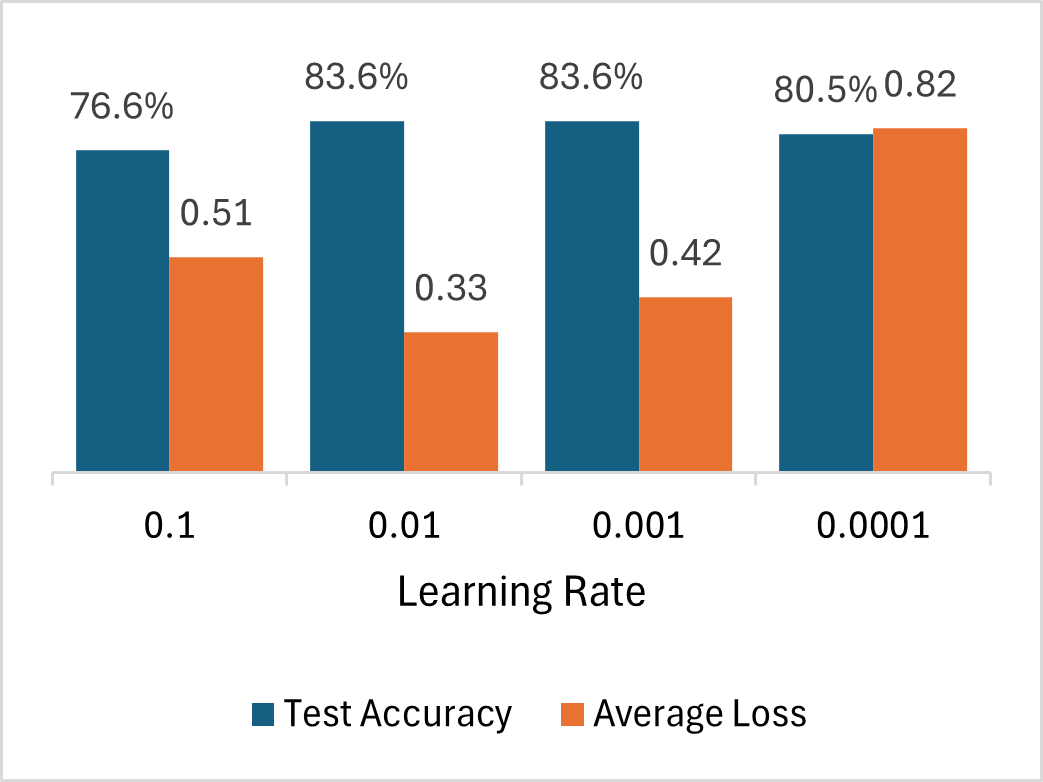
\includegraphics[width=\textwidth]{figure/lr.png}
    \end{minipage}
    \begin{minipage}{0.3\textwidth}
        \centering
        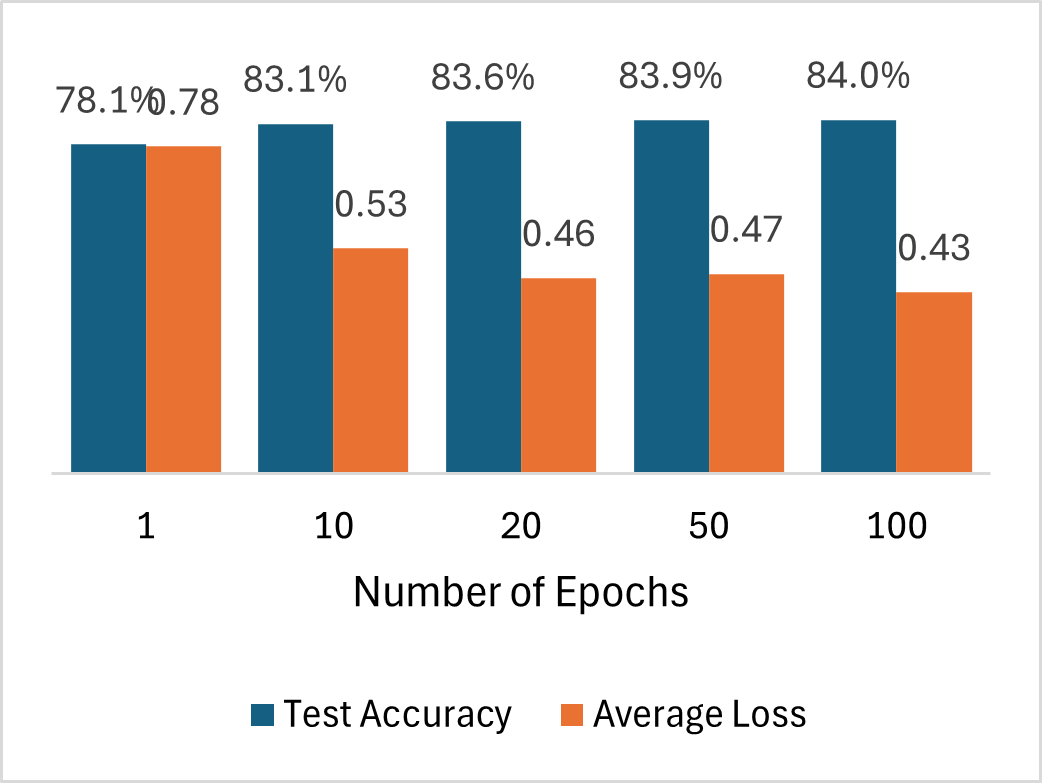
\includegraphics[width=\textwidth]{figure/epoch.png}
    \end{minipage}
    \begin{minipage}{0.3\textwidth}
        \centering
        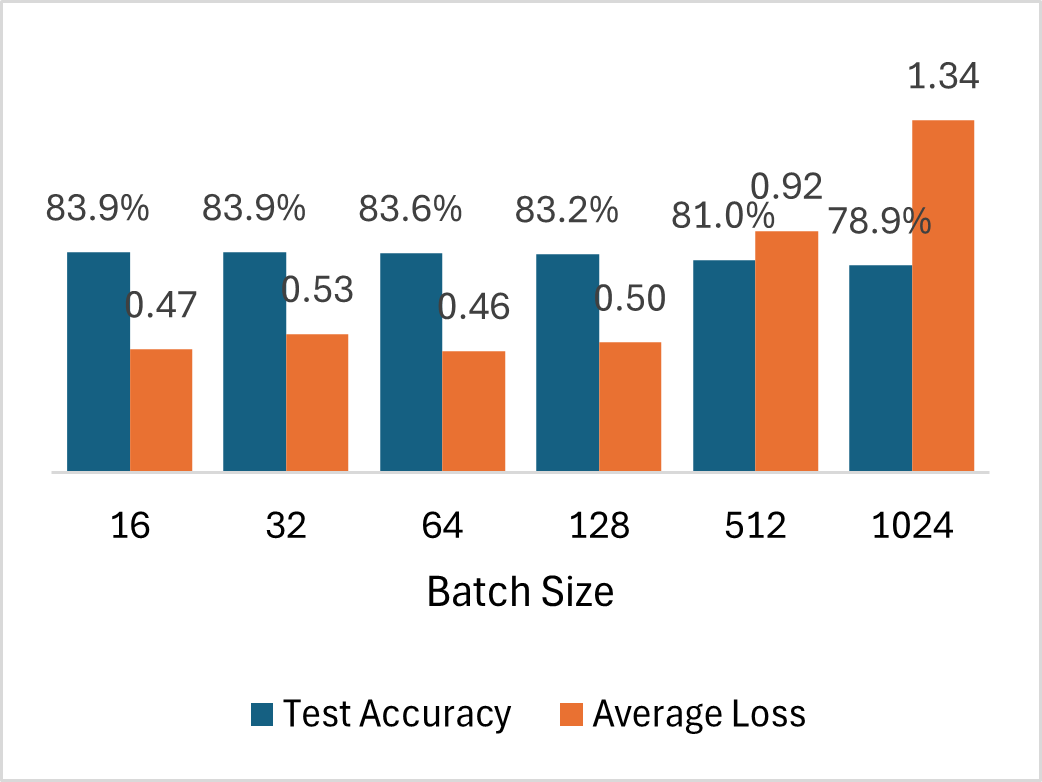
\includegraphics[width=\textwidth]{figure/batch.png}
    \end{minipage}
\end{center}


\textbf{B. Improved Model: } Best Parameters are lr=0.001, ne=20 or 100, bs= 64 or 128, ot=Adam
\begin{center} % Center the images
    \begin{minipage}{0.3\textwidth}
        \centering
        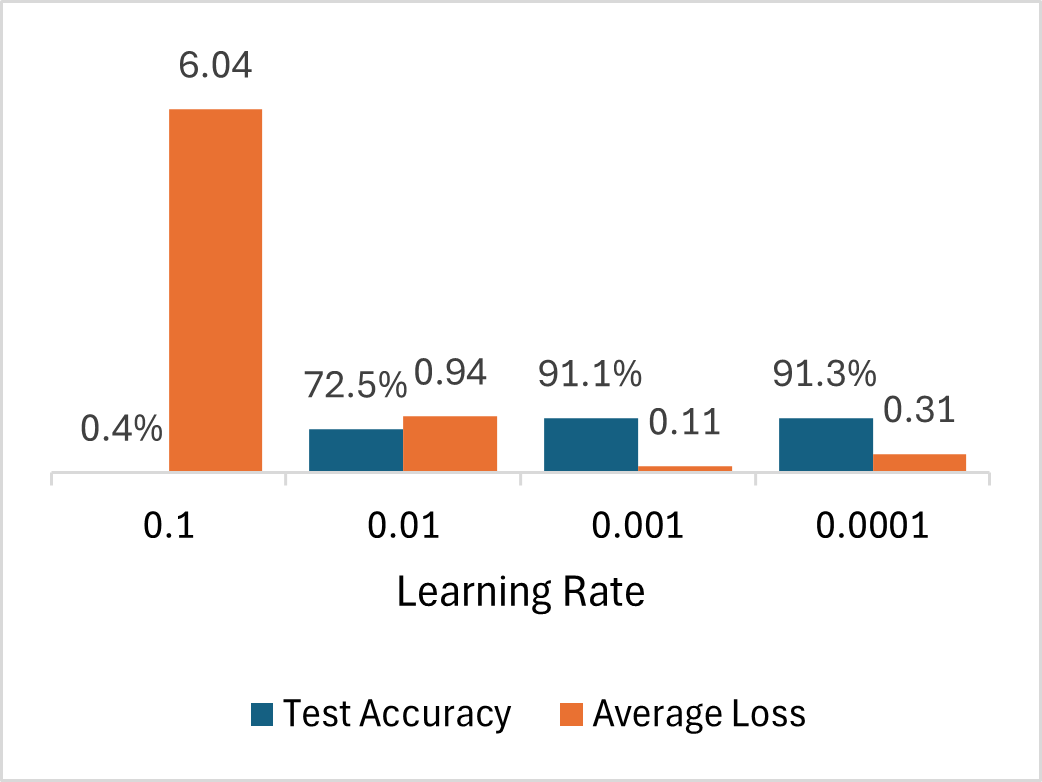
\includegraphics[width=\textwidth]{figure/lr_improved.png}
    \end{minipage}
    \begin{minipage}{0.3\textwidth}
        \centering
        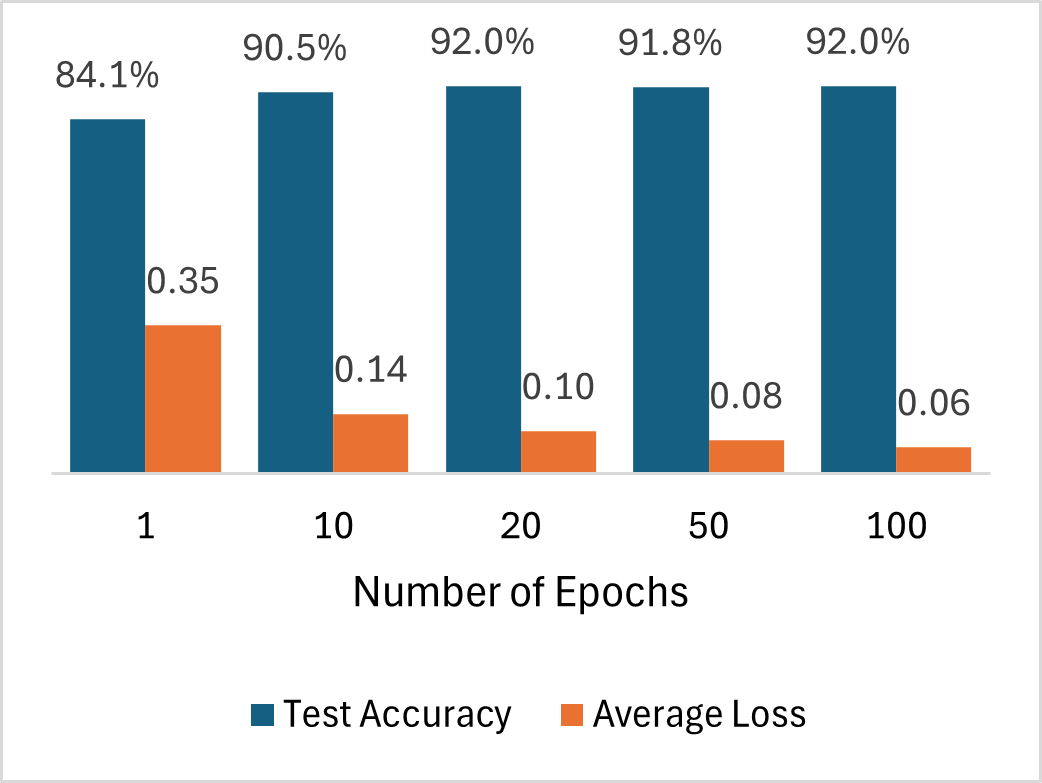
\includegraphics[width=\textwidth]{figure/epoch_improved.png}
    \end{minipage}
    \begin{minipage}{0.3\textwidth}
        \centering
        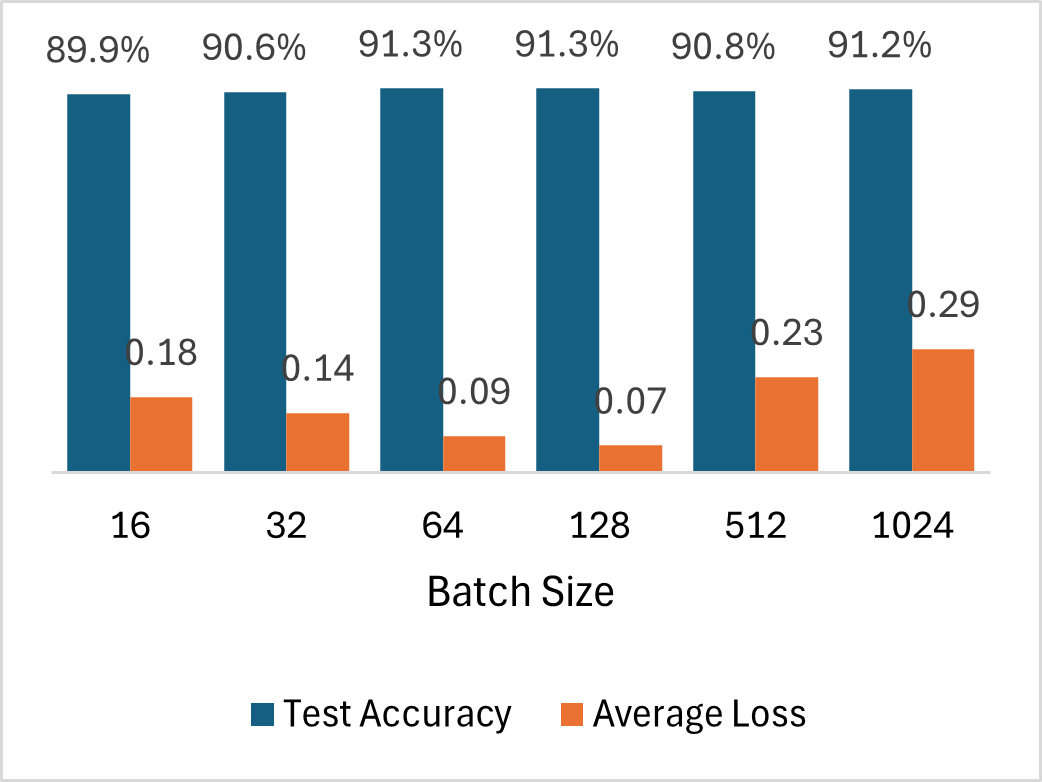
\includegraphics[width=\textwidth]{figure/batch_improved.png}
    \end{minipage}
\end{center}
* for the complete details, please see \href{run:https://git.cs.usask.ca/matcrunch/cmpt-423-820-w25-p2/-/raw/solution/baseline_outputs.txt?ref_type=heads}{\texttt{baseline\_outputs.txt}} and \href{run:https://git.cs.usask.ca/matcrunch/cmpt-423-820-w25-p2/-/raw/solution/improved_outputs.txt?ref_type=heads}{\texttt{improved\_outputs.txt}} for all outputs, and \href{run:https://git.cs.usask.ca/matcrunch/cmpt-423-820-w25-p2/-/blob/solution/summary.pdf?ref_type=heads}{\texttt{summary.pdf}} for a summary of findings.


\subsection{Comparison with the Baseline} 
For the final performance comparison between the improved model and the base model using the central limit theorem, we chose a set of best performing hyper parameters for both and ran each model 10 time (We could have ran more times but that was beyond our time and computation power contraints). 
Then we calculated the average of each of the 10 sets accuracies. And finally we calculated the SEM value for each average that resulted in the 68 percent likely range of accuracies. By observing the gap these two ranges we can confirm that our CNN model has statistically significant improvement than our baseline model:


\begin{table}[htbp]
  \centering
  \begin{tabular}{lccc}
    \toprule
    Model & Mean Accuracy & SEM & 68\% Confidence Interval ($Mean \pm SEM$) \\
    \midrule
    Baseline  & 83.849 & 0.0099 & [83.839, 83.859] \\
    Improved  & 91.111 & 0.0817 & [91.029, 91.193] \\
    \bottomrule
  \end{tabular}
  \caption{Performance Comparison of Baseline and Improved Models}
  \label{tab:performance}
\end{table}

Best hyper parameters used:

Baseline: [Epoch: 20], [LR: 0.001], [Batch: 32], [Optimizer: SGD]

Improved: [Epoch: 20], [LR: 0.001], [Batch: 64], [Optimizer: Adam]





\section{How to Run The Code and Reproduce experiments}
Open the p2/formula.py and follow the instructions at the top of the file to change the desired parameters. See \href{run:https://git.cs.usask.ca/matcrunch/cmpt-423-820-w25-p2/-/blob/solution/summary.pdf?ref_type=heads}{\texttt{summary.pdf}} to find the desired settings and compare results. To run the code, open terminal and go to root directory and call one of these commands:

\subsection{To train and test baseline model:}

\begin{minted}{bash}
$ python p2/formula.py train-baseline
\end{minted}
\subsection{To train and test the improved model:}
\begin{minted}{bash}
$ python p2/formula.py train-improved
\end{minted}
\subsection{To run the the performance comparisons:}
The performance statistics output will be saved to a file called performance\_stats.txt
\begin{minted}{bash}
$ python p2/formula.py performance-diff
\end{minted}
\end{document}

\maketitle

\section{Introduction}

\end{document}
